\documentclass[11pt,letterpaper]{article}
\usepackage{acl2016}
\usepackage{times}

\usepackage{url}
\usepackage{latexsym}
\usepackage{booktabs}
\usepackage{multirow}
\usepackage{graphicx}
\usepackage{paralist}
\usepackage{mathtools}
\usepackage{dingbat}
\usepackage{subcaption}
\usepackage{balance}
\usepackage{gensymb}
\usepackage{marginnote}
\usepackage{adjustbox}

\makeatletter
\newcommand{\@BIBLABEL}{\@emptybiblabel}
\newcommand{\@emptybiblabel}[1]{}
\makeatother
\usepackage{hyperref}

\sloppy

\usepackage{color}
\newcommand{\todo}[1]{}
\renewcommand{\todo}[1]{{\color{red} TODO: {#1}}}

%\renewcommand{\baselinestretch}{0.95}

%\setlength\titlebox{5cm}

% You can expand the titlebox if you need extra space
% to show all the authors. Please do not make the titlebox
% smaller than 5cm (the original size); we will check this
% in the camera-ready version and ask you to change it back.


\title{\ldots}

% \author{First Author \\
%   Affiliation / Address line 1 \\
%   Affiliation / Address line 2 \\
%   Affiliation / Address line 3 \\
%   {\tt email@domain} \\\And
%   Second Author \\
%   Affiliation / Address line 1 \\
%   Affiliation / Address line 2 \\
%   Affiliation / Address line 3 \\
%   {\tt email@domain} \\}

\date{}

\newcommand{\BASEURL}{http://example.org}
% \newcommand{\BASEURL}{https://bitbucket.org/dimazest/phd-buildout/raw/tip/notebooks/downloads/compdistmeaning}
\newcommand{\dataurl}[1]{\href{\BASEURL/#1}{\nolinkurl{#1}}}

\newcommand{\p}{\textsuperscript{\textasteriskcentered}}
\newcommand{\pw}{\textsuperscript{\dag}}

\newcommand{\pp}{\textsuperscript\dag}
\newcommand{\ppp}{\textsuperscript\ddag}
\newcommand{\np}{\phantom{\textsuperscript\textasteriskcentered}}

\def\relevant/{Relevant@3}
\def\topRR/{Top Reciprocal Rank}
\def\RR/{Reciprocal Rank}


\begin{document}
\def\emnlp/{\textit{KS2013}}
\def\PhraseRel/{PhraseRel}

\def\PMI/{$1 \operatorname{PMI}$}
\def\SPMI/{$1 \operatorname{SPMI}$}
\def\CPMI/{$1 \operatorname{CPMI}$}
\def\SCPMI/{$1 \operatorname{SCPMI}$}

\def\NPMI/{$n \operatorname{PMI}$}
\def\NSPMI/{$n \operatorname{SPMI}$}
\def\NCPMI/{$n \operatorname{CPMI}$}
\def\NSCPMI/{$n \operatorname{SCPMI}$}

\def\logNPMI/{$\log n\operatorname{PMI}$}
\def\logNSPMI/{$\log n\operatorname{SPMI}$}
\def\logNCPMI/{$\log n \operatorname{CPMI}$}
\def\logNSCPMI/{$\log n \operatorname{SCPMI}$}


\maketitle
\begin{abstract}
Previous optimisations of parameters affecting the word-context association measure used in distributional vector space models have focused on high-dimensional vectors; but low-dimensional versions are often required in compositional tasks. We present a systematic study of the interaction of these parameters and vector dimensionality, and derive parameter selection heuristics that achieve performance across different datasets competitive with the results previously reported in the literature.

\end{abstract}

\section{Introduction}
\label{sec:introduction}

Vector space models of language were inspired by the idea of \newcite{harris1954distributional} and \newcite{firth1957lingtheory} that meanings of words can be deduced from their co-occurrence with other words in natural text. If a word co-occurs with a context word more often than can be expected, this context word is indicative of the word's meaning, while the opposite indicates disjointness in meaning.
\newcite{Dagan:1993:CWS:981574.981596} were among the first to apply this idea computationally and to represent word meaning by an ordered range of values of
\emph{mutual information}\footnote{Also known as pairwise or pointwise mutual information and commonly abbreviated as PMI.} \cite{church1990word}.
Each value expresses the ratio between the observed and the expected co-occurrence, and, therefore, measures the association of the target word with a reference word. A word could thus be expressed as a vector with a set of contextual terms as its features, and as their weights a measure of association. This idea forms the basis of distributional semantics and has become mainstream in information retrieval and natural language processing tasks.

Over the last decades, various information-theoretic alternatives and refinements to mutual information have been introduced to capture lexical semantics. The most notable are \emph{positive PMI} (PosPMI, \newcite{BullinariaLevy07}) and \emph{local mutual information} (LMI, \newcite{evert2008corpora}).
These measures differ from PMI in their treatment of frequencies below expectation, and in the weight assigned to observed frequencies, embodied in additional multiplication factors.

\newcite{TACL570} suggested to optimize PMI with a  set of parameters adopted from predictive models of \newcite{mikolov2013efficient}, most notably \emph{shifted PMI} abbreviated as \texttt{neg} and \emph{context distribution smoothing} referred to as \texttt{cds}. Their experiments and thus the parameter selection recommendations use highly dimensional vector spaces with word vector  dimensionality of almost \textbf{200K}. As such, recent work on lexical distributional semantics with the results close to the state of the art involve vectors with a considerable dimensionality of hundreds of thousands \cite{baroni-dinu-kruszewski:2014:P14-1,kiela-clark:2014:CVSC}.

Contrary to the trend of employing highly dimensional vectors, other work on lexical and compositional distributional semantics employ vectors with much less dimensions, for example, \textbf{2K} \cite{Grefenstette:2011:ESC:2145432.2145580,kartsadrqpl2014,milajevs-EtAl:2014:EMNLP2014}, \textbf{3K} \cite{Dinu:2010:MDS:1870658.1870771,milajevs-purver:2014:CVSC} or \textbf{10K} \cite{polajnar-clark:2014:EACL,Baroni2010nouns}.

Such a mismatch in vector dimensionality selection across lexical and compositional tasks rises a number of questions this paper aims to answer.
\begin{itemize}
\item To what extent does model performance depend on vector dimensionality?
\item Do parameters influence performance of highly dimensional models the same way as lowly dimensional models? Are finding of \newcite{TACL570} directly transferred to lowly dimensional models?
\item Is it possible to come up with the heuristics for model parameter selection? If so, what are they?
\item Can the heuristics based on lexical tasks be transferred to compositional tasks?
\end{itemize}

To answer these questions we perform a systematic study of distributional models with a rich set of parameters on two lexical datasets: SimLex-999 \cite{hill2014simlex} and MEN \cite{Bruni:2014:MDS:2655713.2655714}; and three compositional datasets: KS14 \cite{kartsadrqpl2014}, GS11 \cite{Grefenstette:2011:ESC:2145432.2145580} and PhraseRel.

\section{Parameters}
\label{sec:parameters}

\begin{table}
  \centering
  % \footnotesize
  \begin{tabular}{llc}
    \toprule
    Parameter & Values \\
    \midrule
    \multirow{2}{*}{Dimensionality} & 1K, 2K, 3K, 5K \\
                                    & 10K, 20K, 30K, 40K, 50K \\
    \texttt{discr} & PMI, CPMI, SPMI, SCPMI \\
    \texttt{freq} & $1$, $n$, $\log n$ \\
    \texttt{neg} & 0.2, 0.5, 0.7, 1, 1.4, 2, 5 \\
    \texttt{cds} & \textit{global}, 1, 0.75 \\
    Similarity & Cosine, correlation \\
    Window size & 5                                \\
    \multirow{2}{*}{Corpus} & Concatenation of \\
                            & ukWac and Wackypedia \\
    \bottomrule
  \end{tabular}
  \caption{\textbf{Model parameters and their values.}}
\label{tab:parameters}
\end{table}

%%% Local Variables:
%%% mode: latex
%%% TeX-master: "paper"
%%% End:


\subsection{PMI variants (\texttt{discr})}
\label{sec:pmi-variants}

Co-occurrence weightings schemes based on \emph{Point-wise mutual information} (PMI, Equation~\ref{eq:pmi}) have been successfully applied in distributional semantics (see for example \newcite{J90-1003}, \newcite{Turney:2010:FMV:1861751.1861756} and \newcite{NIPS2014_5477}).
%
\begin{equation}
  \label{eq:pmi}
  \operatorname{PMI}(x, y) = \log\frac{P(x,y)}{P(x)P(y)}
\end{equation}

PMI is not directly applicable to the co-occurrence matrix because non-observed co-occurrences lead to infinite PMI values which in turn make it impossible to compute similarity. A straightforward ``fix'' to this problem is to replace all infinities with zeroes. Such a replacement preserve sparsity of the input co-occurrence matrix. Later in the paper, we use PMI to refer to a weighting with this fix.

An alternative solution of avoiding infinity is to increment the probability ratio by one:
%
\begin{equation}
  \label{eq:cpmi}
  \operatorname{CPMI}(x, y) = \log\Big( 1 + \frac{P(x,y)}{P(x)P(y)} \Big)
\end{equation}

\subsection{Shifted PMI (\texttt{neg})}
\label{sec:shifted-pmi}

It has been experimentally shown that negative PMI values do not positively contribute to model performance and worth nullifying \cite{Turney:2010:FMV:1861751.1861756}. Positive PMI extended with an additional additional hyperparameter $k$ (\texttt{neg}) following \newcite{TACL570} is the third PMI variant (abbreviated as SPMI) used in this work:
%
\begin{equation}
  \label{eq:ppmi}
  \operatorname{SPMI_k} = \max (0, \operatorname{PMI}(x, y) - \log k)
\end{equation}
%
As $k$ increases, more values become 0 and, consequently, vectors become sparser. Setting $k$ to 1 is equivalent to vanilla positive PMI without shifting. When $k < 1$ vectors are denser.

Finally, we can apply the same idea to CPMI:
%
\begin{equation}
  \label{eq:pcpmi}
  \operatorname{SCPMI_k} = \max (0, \operatorname{CPMI}(x, y) - \log 2k)
\end{equation}

\subsection{Frequency weighting (\texttt{freq})}
\label{sec:frequency-weighting}

Another issue with PMI is its bias towards rare events \cite{TACL570} one way of solving this issue is to weight PMI value by the co-occurrence frequency \cite{Evert05}:
%
\begin{equation}
  \label{eq:lmi}
  \operatorname{LMI}(x, y) = n(x, y)\operatorname{PMI}(x, y)
\end{equation}
%
where $n(x, y)$ is the number of times $x$ was seen together with $y$. For clarity, we refer to $n$ weighted PMIs as \NPMI/, \NSPMI/ \NCPMI/ and \NSCPMI/. When frequency component is set to 1, it does not have an effect giving rise to explicit quantification labels: \PMI/, \SPMI/, \CPMI/ and \SCPMI/.

In addition to $1$ and $n$ frequencies, we experiment with $\log n$ frequency.

\subsection{Context distribution smoothing (\texttt{cds})}
\label{sec:cont-distr-smooth}

Context distribution smoothing (\texttt{cds}) is another parameter shown to influence performance of distributional models \cite{TACL570}. It smoothes the context distribution $P(x)$:
%
\begin{equation}
  \label{eq:cds}
  P_{\alpha}(x) = \frac{n(x)^{\alpha}}{\sum_{c}n(c)^{\alpha}}
\end{equation}
%
We experiment with values of 1 (absence of smoothing) and 0.75 and sometimes refer to such context probability estimation as \emph{local context probability}.

We also estimate probability of a context using the global context appearance in the corpus:
%
\begin{equation}
  \label{eq:cds-nan}
  P(x) = \frac{n(x)}{|C|}
\end{equation}
%
where $|C|$ is the size of the used corpus. We refer to this case as \emph{global context probability}.

\begin{figure*}[ht]
  \centering
  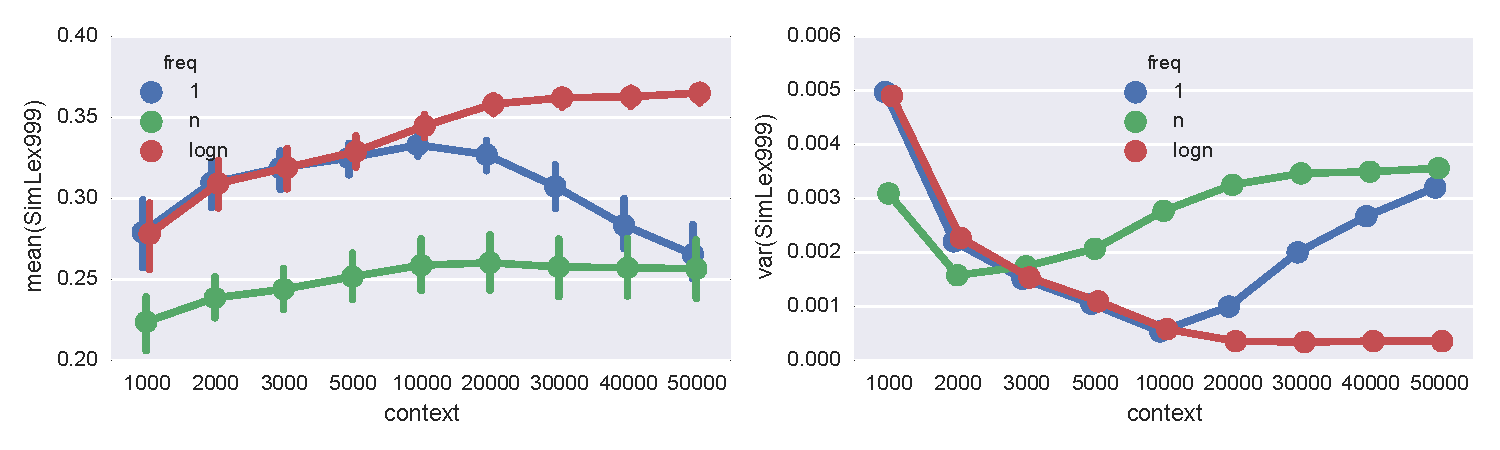
\includegraphics[width=\textwidth]{supplement/figures/simlex-ppmi}
  \caption{\textbf{Shifted PMI mean performance and variance.}}
  \label{fig:ppmi-performance}
\end{figure*}

\subsection{Vector dimensionality}
\label{sec:vect-dimens}

As context words we select 1K, 2K, 3K, 5K, 10K, 20K, 30K, 40K and 50K most frequent lemmatised nouns, verbs, adjectives and adverbs. All context words are part of speech tagged, but we do not make difference between refined word types, for example, we do not distinguish between transitive and ditransitive verbs.

\subsection{Similarity metric}
\label{sec:similarity-metric}

We test a widely used cosine based similarity, as well as correlation \cite{kiela-clark:2014:CVSC}.

\subsection{Compositional operator}
\label{sec:comp-oper}

For tasks that involve composition, we test the following operators: \textbf{addition}
and \textbf{multiplication} \cite{mitchell2010composition}; \textbf{Kronecker} \cite{Grefenstette:2011:ETV:2140490.2140497}; \textbf{Relational} \cite{Grefenstette:2011:ESC:2145432.2145580}; \textbf{Copy object} and \textbf{Copy subject} \cite{Kartsaklis12aunified}; \textbf{Frobenius addition}, \textbf{Frobenius multiplication} and \textbf{Frobenius outer} \cite{kartsadrqpl2014}.

Table~\ref{tab:parameters} lists the parameters and their values used in this work.

\section{Lexical experiments}
\label{sec:lexical-experiments}

Figure~\ref{fig:ppmi-performance} shows the mean performance and the variance of the SPMI models grouped by vector dimensionality and frequency on the SimLex-999 dataset.

We start with exploring the performance of \SPMI/. Average \SPMI/ performance increases for the dimensionality values in the range of 1K to 10K. After 10K dimensions, the average \SPMI/ performance degrades. \SPMI/ score variance is the smallest for the 10K dimensional models and it grows as the dimension number increases afterwards. This suggests that there are particular parameter combinations that weaken or strengthen the results of the lowly and highly dimensional models.

Interestingly, \logNSPMI/ mean performance increases and variance decreases as dimensionality increases showing that this weighting is not sensitive to the parameter selection for highly dimensional models.

\paragraph{Parameter interaction}

\begin{figure*}
  \centering
  \begin{subfigure}[b]{\textwidth}
    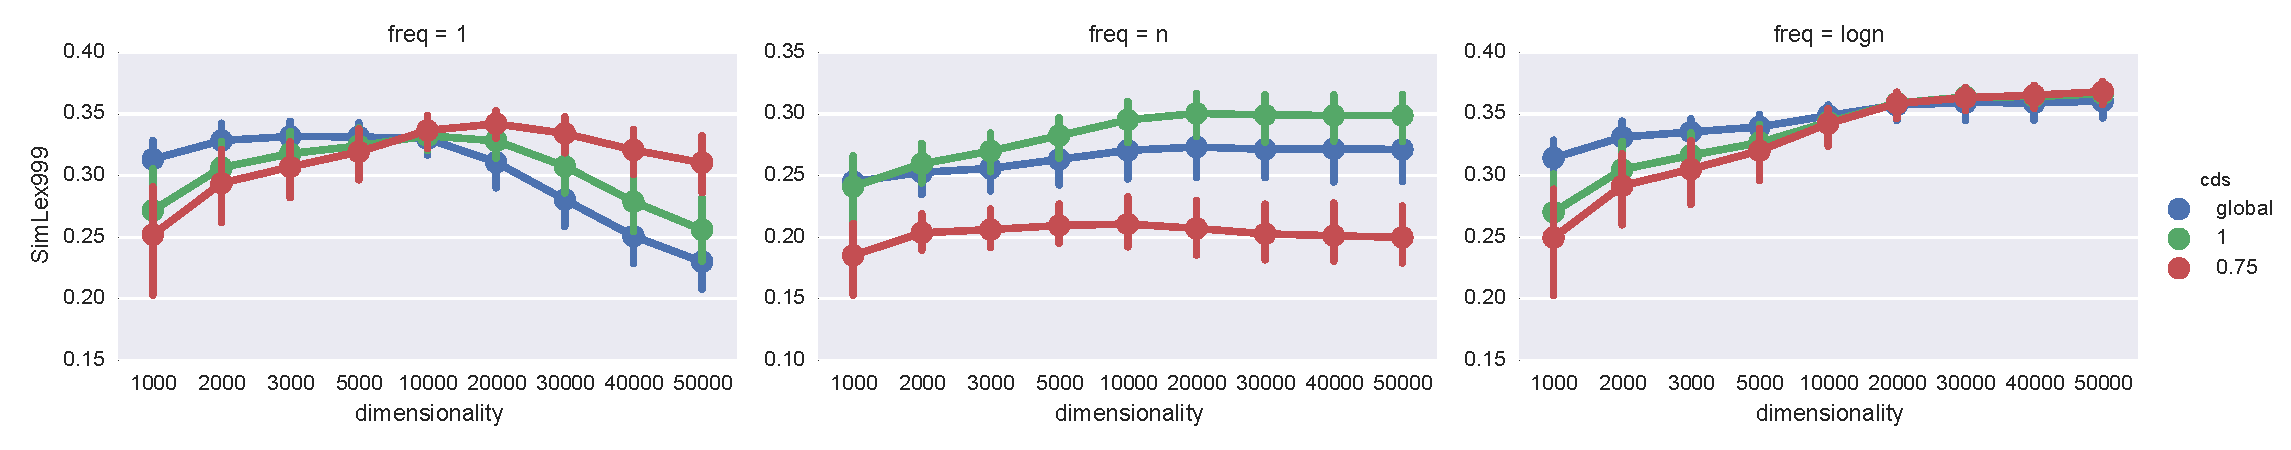
\includegraphics[width=\textwidth]{supplement/figures/simlex-ppmi-cds.pdf}
    \caption{\textbf{Context distribution smoothing.}}
    \label{fig:simlex-ppmi-interaction-cds}
  \end{subfigure}

  \begin{subfigure}[b]{\textwidth}
    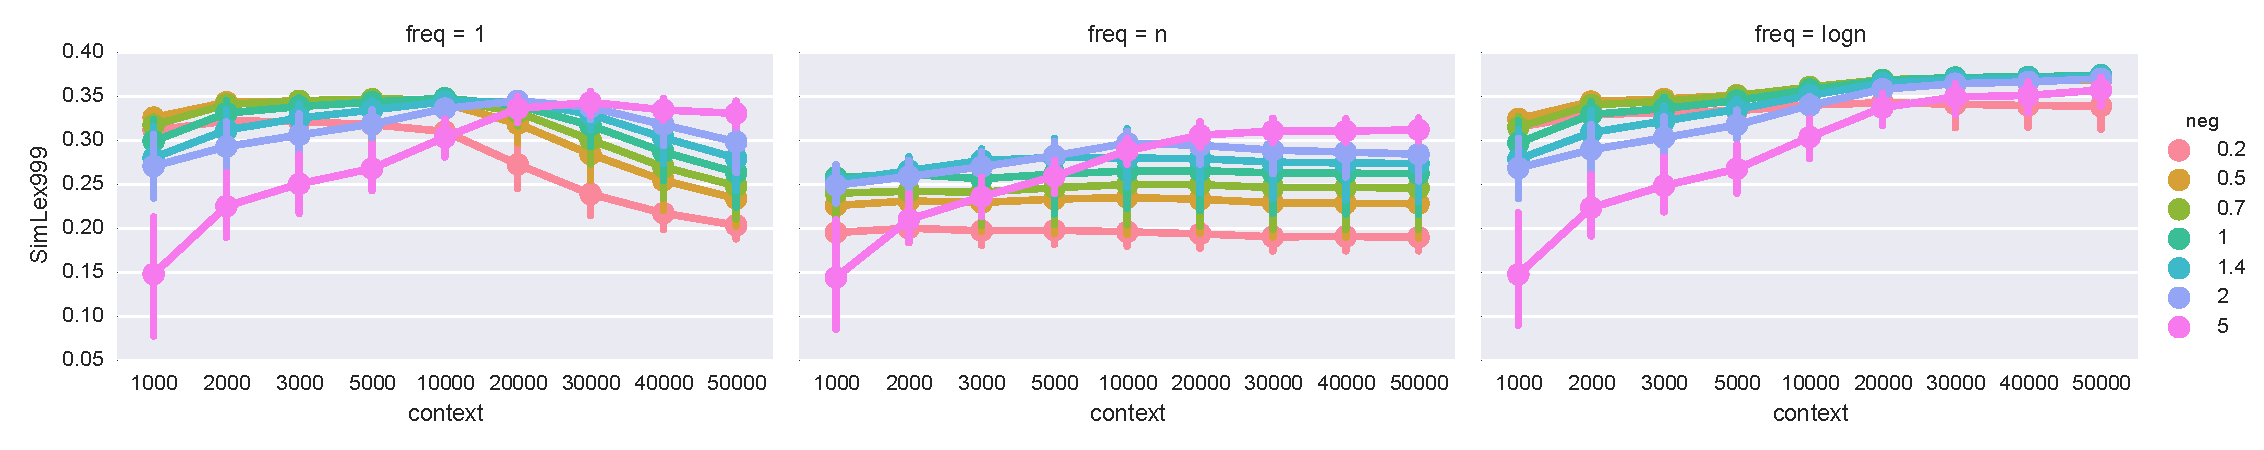
\includegraphics[width=\textwidth]{supplement/figures/simlex-ppmi-neg.pdf}
    \caption{\textbf{Shifting.}}
    \label{fig:simlex-ppmi-interaction-neg}
  \end{subfigure}

  \caption{\textbf{SPMI.}}
  \label{fig:simlex-ppmi-interaction}
\end{figure*}

%%% Local Variables:
%%% mode: latex
%%% TeX-master: "paper"
%%% End:


Figure~\ref{fig:simlex-ppmi-interaction} shows dimensionality-\texttt{cds} and dimensionality-\texttt{neg} parameter interactions. 10K dimensional \SPMI/ is, indeed, the least sensitive to parameter selection. For models with dimensionality greater than 10K, context distribution smoothing should be used with $\alpha = 0.75$. For models with dimensionality lower than 10K, it is beneficial to use global context probabilities. Shifting also depends on the dimensionality, models with up to 3K dimensions should set $k = 0.5$, models with up to 30K dimensions should set $k = 1.4$ and models with a higher number of dimensions should set $k = 2$.

\logNSPMI/ should be used with global context probabilities for models with vector dimensions up to 10K. For more dimensional spaces, smoothing should be applied with $\alpha = 0.75$. Shifting should be applied with $\alpha = 0.5$ for models with less than 10K dimensions and $\alpha = 1.4$ for models with more than 10K dimensions.

\NSPMI/ gives good results with local context probabilities ($\alpha = 1$), models with less than 20K dimensions should be used with $k = 1$, otherwise $k = 1.4$ should be preferred.

We use correlation similarity metric for \SPMI/ and \NSPMI/ based models, cosine similarity is used for \logNSPMI/.

The proposed heuristics work well for \logNSPMI/, where performance variance is low, the performance of models selected using the heuristics is not lower than 0.01 point of the best configuration. For \SPMI/ and \NSPMI/ this difference is much higher, refer to Figure~\ref{fig:simlex-ppmi-best-simlex} for more details.

Finally, to see whether the heuristics are applicable to other datasets, we contrast the selected models with the best scores on the MEN dataset (see Figure~\ref{fig:simlex-ppmi-best-men}). Again, \logNSPMI/ follows the best possible setup closely, especially for models with the dimension number greater than 10K. Surprisingly, the heuristics for \NSPMI/ are very effective on the MEN dataset, even though they are based on SimLex-999. Heuristics for \SPMI/ do not guarantee best possible results.

In general, model performance depends on vector dimensionality (the best setup with 50K dimensions is better than the best setup with 1K dimensions by 0.03 on SimLex-999). It is beneficial to experiment with dense and unsmoothed low dimensional spaces ($k < 1$, global context probability); and sparse and smooth high dimensional spaces ($k > 1$, $\alpha = 0.75$). However, these heuristics do not guarantee the best possible result for \SPMI/ and \NSPMI/ because of high variance of the corresponding scores. Based on this we suggest to use \logNSPMI/ with the dimensionality of at least 20K to ensure good performance on lexical tasks.

\begin{figure*}
  \centering
  \begin{subfigure}[b]{\textwidth}
    \includegraphics[width=\textwidth]{supplement/figures/SimLex999-ppmi-best.pdf}
    \caption{SimLex-999}
    \label{fig:simlex-ppmi-best-simlex}
  \end{subfigure}


  \begin{subfigure}[b]{\textwidth}
    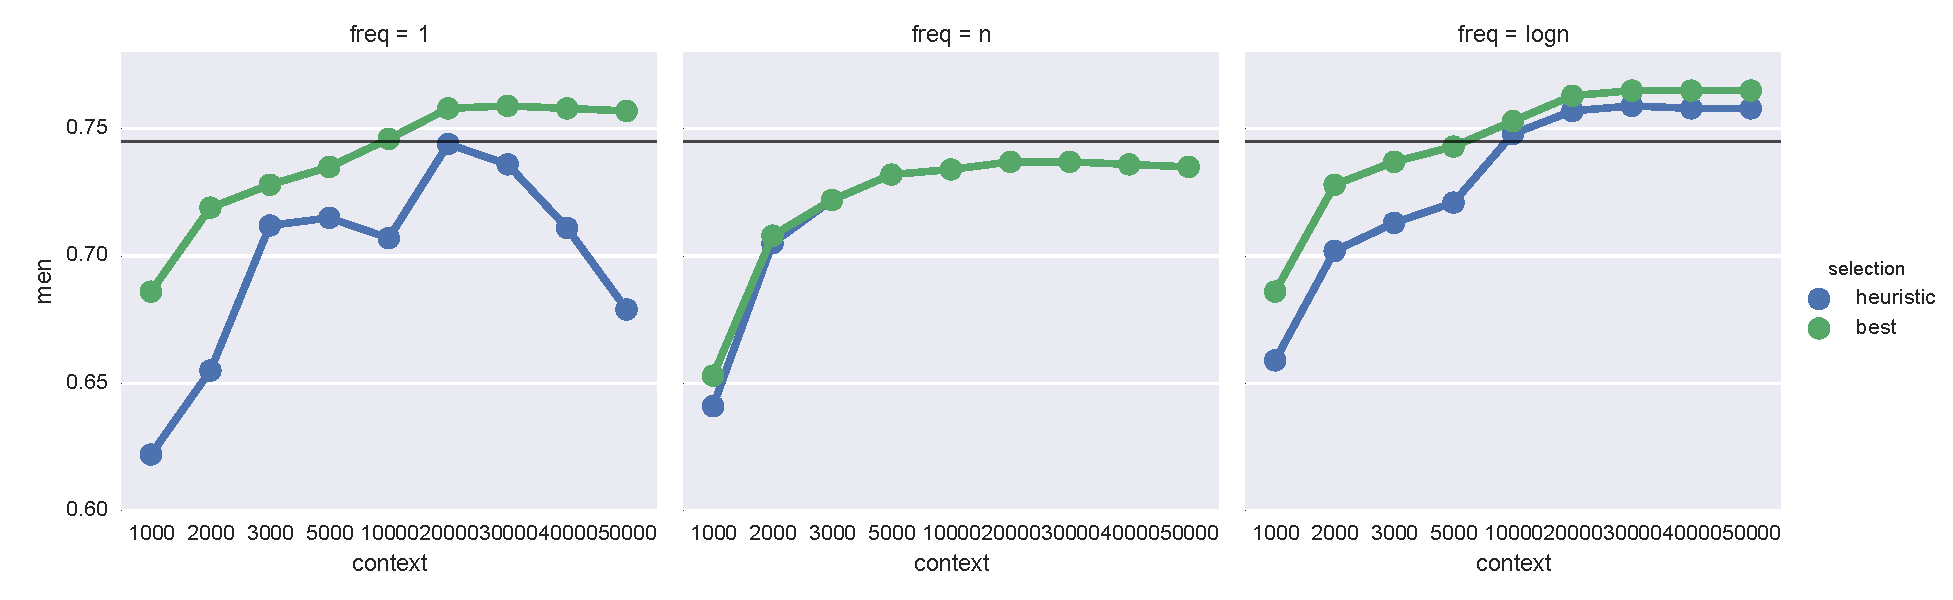
\includegraphics[width=\textwidth]{supplement/figures/men-ppmi-best.pdf}
    \caption{MEN}
    \label{fig:simlex-ppmi-best-men}
  \end{subfigure}

  \caption{\textbf{SPMI best configurations.} Black line shows the best results reported by \protect\newcite{TACL570}.}
  \label{fig:simlex-ppmi-best}
\end{figure*}

%%% Local Variables:
%%% mode: latex
%%% TeX-master: "paper"
%%% End:


\section{Compositional experiments}
\label{sec:compositional-experiments}

\begin{figure*}
  \centering
  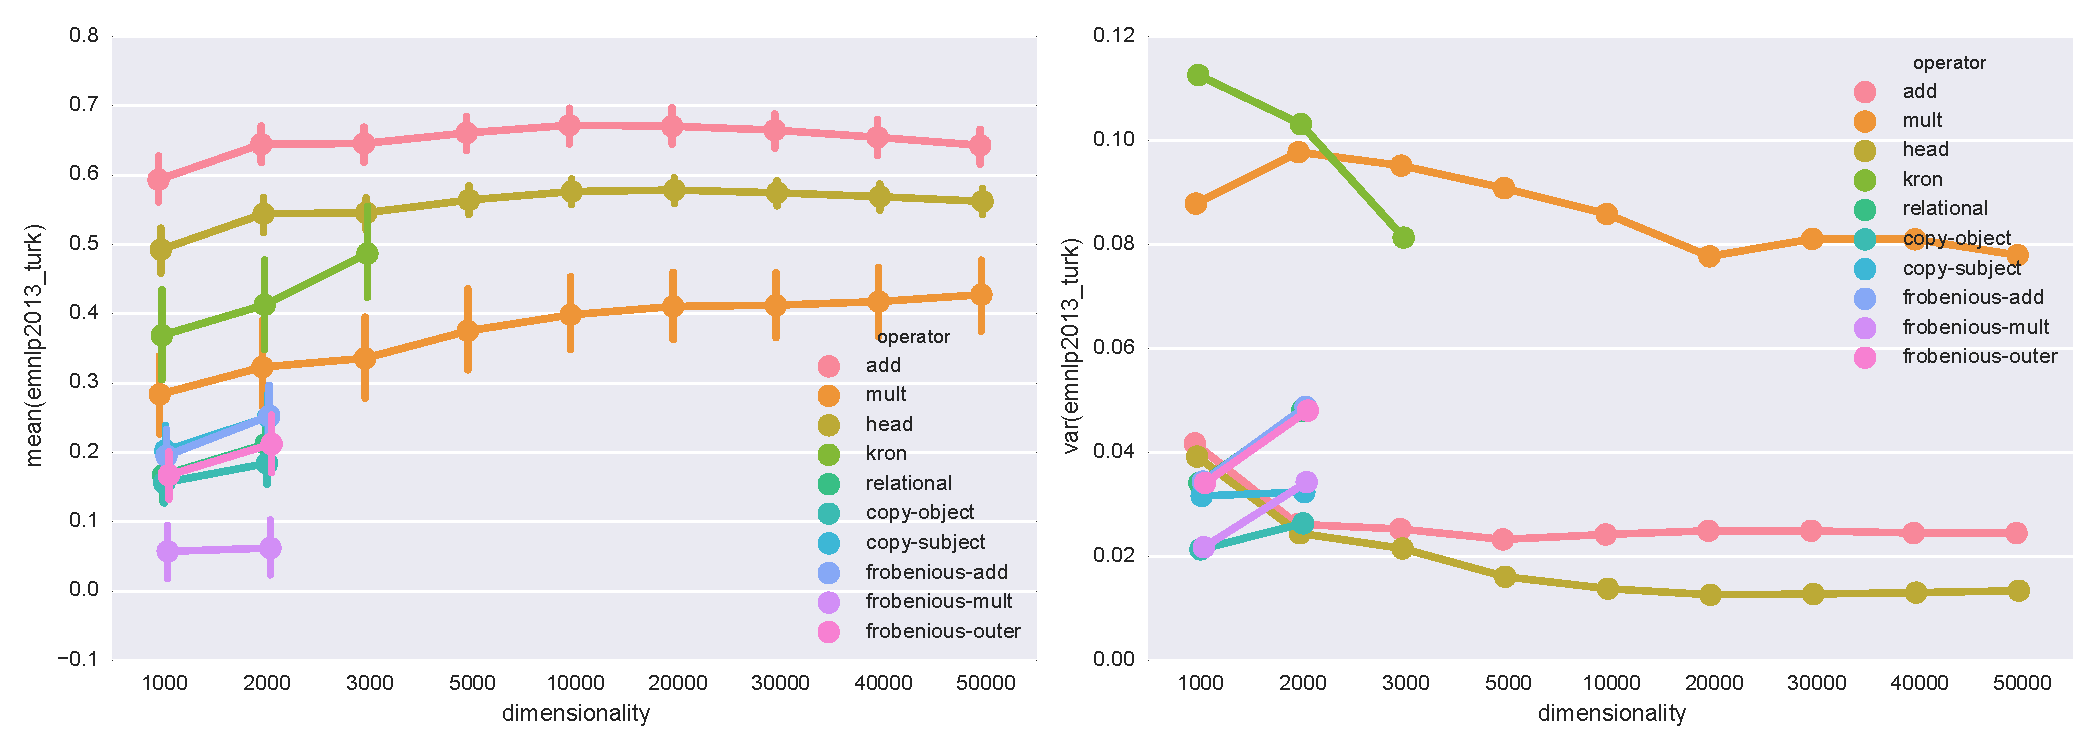
\includegraphics[width=\textwidth]{supplement/figures/emnlp13-ppmi-performance}
  \caption{\textbf{Shifted PMI mean performance and variance on the EMNLP13 dataset.}}
  \label{fig:emnlp13-ppmi-performance}
\end{figure*}


In compositional experiments, the main goal is to study compositional operators rather than special weighting schemes, therefore we will see the weighting scheme as another hyperparameter that is being optimized and study compositional operators in isolation.

Figure~\ref{fig:emnlp13-ppmi-performance} shows SPMI's average performance and evaluation score variance on the KS14 dataset.

Addition has the highest average performance and a relatively low variance. Multiplication, shows lowest average performance, but the result variance is much higher than addition. Kronecker exhibits behavior similar to multiplication.

\subsection{Addition}
\label{sec:addition}





%\bibliographystyle{acl}
% remove publisher, month etc from conf proceedings:
\bibliographystyle{acl-short}
% \bibliographystyle{naaclhlt2016}
\balance
\bibliography{references,dmilajevs_publications}

\end{document}
